\documentclass{jfsma}
\usepackage{lmodern}
\usepackage{hyperref}
\usepackage{caption}
\usepackage{cuted}
\usepackage{etoolbox}

\titre{Automatic Observer For Real-Time Strategy Games} % On garde ce titre ?
\auteur{Emmanuel \textsc{Hadoux}}{emmanuel.hadoux@lip6.fr}
\auteur{Thomas \textsc{Huraux}}{thomas.huraux@lip6.fr}
\institution{
  LIP6, CNRS UMR 7606,\\
  Universit\'e Pierre et Marie Curie, Paris, France}

\begin{document}
	\maketitle
	
	\begin{strip}
  \centering\noindent
  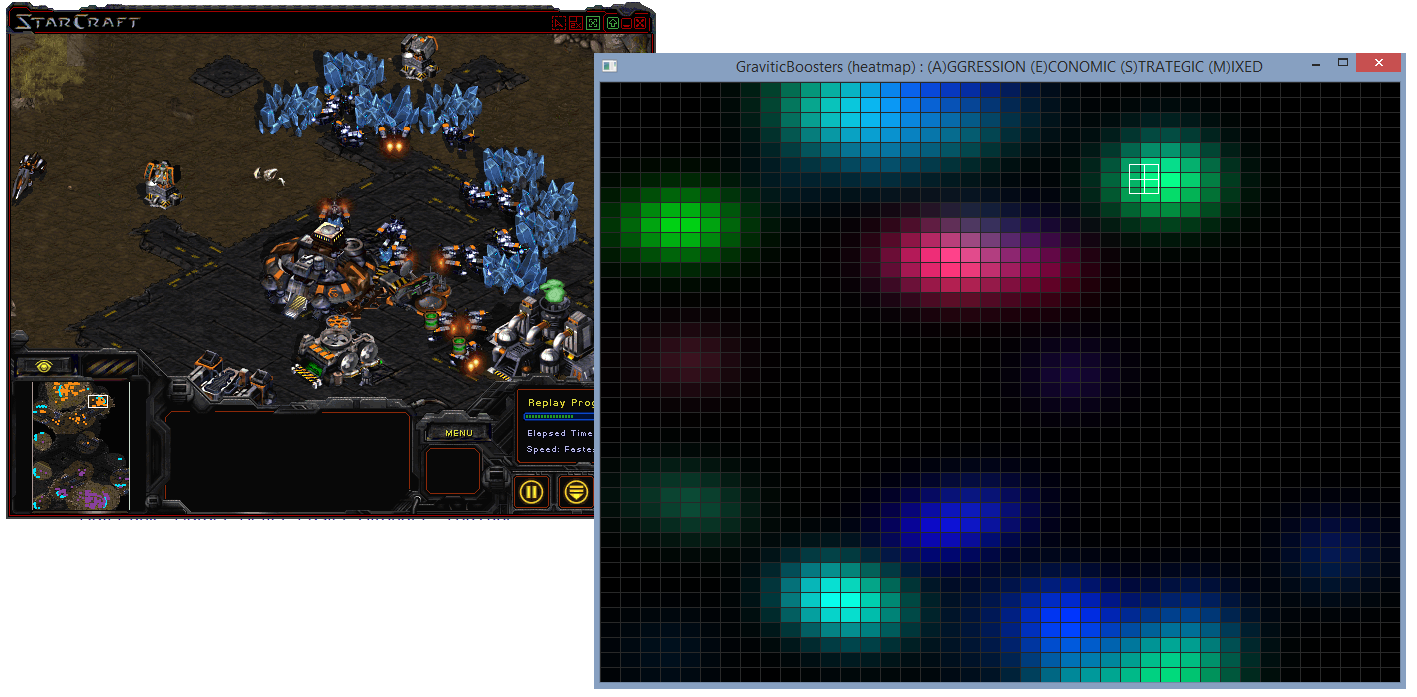
\includegraphics[scale=0.35]{gfx/GB}
  \vspace{0.3cm}
\end{strip}

	\section{Context}
    	Electronic sport (\textit{e-sport}) is a not-so-young discipline slowly growing in western countries.
        It took root in South-Korea about 15 years ago and is currently experiencing an explosion of interest.
        The first game entering the closed category of e-sport was Starcraft 1. % T: faut voir si on parle tout de suite de SC ou alors on vise un truc plus générique
        This fast-paced real-time strategy game (\textit{RTS}) was released in 1998.
	Since then RTS games challenge many research works in AI such as planning in resource allocation, force deployment, and battle tactics~\cite{weber2009case,mccoy2008integrated}; spatial reasoning~\cite{forbus2002qualitative} or opponent modeling~\cite{schadd2007opponent}.
        
        During battles between the two armies, players can reach picks of 450 actions-per-minutes (\textit{APM}).
        For obvious related reasons, viewers cannot follow the game by watching the screens of the players.
        Competitions thus require an external observer following the game and showing important actions.
        However, being an observer requires a comprehensive knowledge of the game as well as anticipation and entertainment faculties. 
        Few persons are able to gather all those skills, making them even more famous than some professional players.
        
        In this work, we propose an automatic observer able to catch every piece of action to assist or replace the human observer. The following breafly describes our approach to answer this problem.
        
\section{Overview of the method}
We set ourselves two constraints to the realization of an automatic observer: on one hand real time calculation to be used in the context of a real game with pro players, and on the other hand, to use only standard information that can be found in any RTS (position, unit price, damage, ...).

Each entity (unit or building) has three potentials computed in real time during the game:\\
\textsc{aggressive potential} allows to anticipate the interest of an upcoming fight by taking into account the distance to the enemy and the damage per second (\emph{DPS})\\
\textsc{economic potential} informs on base creation, workers training, etc.\\
\textsc{strategic potential} shows information-taking units (called \emph{scoot}) 

Those three features are the most important side of a competitive RTS game.
Indeed, players need workers and bases to gather resources allowing them to make units to build an army.
However, as they cannot train workers and units at the same time, they need to choose to go agressive or economic based on gathered strategic information.
The purpose of this model is to show where and when those choices are made and thus complementing the work of the casters (the commentators).

To that end, the map is discretized so that each cell aggregates the potentials of all entities composing it. The camera is then simply positioned at the maximum value of the resulting matrix.
To enhance position on the game's action, we smooth the potential matrix using a gaussian kernel. 
This allows, for instance, to position the camera between two armies facing each other. 

We also added two dynamic parameters to the camera: \emph{commitment} and \emph{weariness} in order to limit both disturbing too-frequent changes and over-attention to the same area.

\section{Implementation}

Based on this method, we develop an automatic observer called \emph{Gravitic Boosters}\,\footnote{\url{http://github.com/EHadoux/GraviticBoosters}}.
We tested our approach on Starcraft Broodwar\,\footnote{\url{http://us.blizzard.com/en-us/games/sc/}} using
the BWAPI API~\cite{bwapi} which enables to retrieve all current information and to take control of both the units and the game interface.
As a side note, this API has been used for 5 years in several StarCraft AI Competitions, supported by the University of Alberta\,\footnote{\url{http://webdocs.cs.ualberta.ca/~cdavid/starcraftaicomp/}}.

The figure above shows a Starcraft game and a corresponding visualization of the three potentials as a heat map. 
RGB colors are used to encode the three components: red represents the aggressive potential, green the economic potential and blue the strategic one.

\section{Perspectives}
We consider several perspectives in the context of our work...

The video game industry continues to expand as very little AI has been involved in this expansion~\cite{miikkulainen2007creating}. Especially since AI is not a priority of publishers compared to \textit{e.g.} graphics with a better marketing value. Nevertheless, we believe that AI can bring more to this media as we try to illustrate with our work presented in this paper. Especially in esport where some competitions have now over 10.000.000\$ in prize money and where stadiums are under construction.
We argue that research should be encouraged to take advantage of this recent expansion.

\bibliographystyle{plain}
\bibliography{biblio}

\end{document}
